\documentclass[11pt]{beamer}
\usepackage{multicol}
\usetheme{Warsaw}

%\definecolor{applegreen}{rgb}{0.55, 0.71, 0.0}
%\usecolortheme[named=applegreen]{structure}

\title{Program Analysis - Herbrand Equivalence}
\subtitle{MidTerm BTP Presentation}

\author{Himanshu Rai}
\institute{Indian Institute of Technology, Palakkad}
\date{24/09/2019}

\begin{document}

\begin{frame}
\titlepage
\end{frame}

\begin{frame}{Optimizing Compilers}
    \begin{itemize}
        \item Modern compilers perform a lot of optimizations on the code
        \item One common optimization performed is detecting equivalence of program subexpressions
        \item It is the main theme of many algorithms like constant propagation, constant folding, common subexpression elimination etc.
        \item Each of these detect a restricted class of expression equivalence
        \item In fact checking equivalence of program subexpressions have been shown to be an undecidable problem
        \item Informally, this means we can't have an algorithm to find all equivalent subexpressions in a program
    \end{itemize}
\end{frame}

\begin{frame}{Herbrand Equivalence}
    \begin{itemize}
        \item So, usually a restricted form of expression equivalence called \textit{Herbrand Equivalence} is targetted
        \item Two expressions are Herbrand equivalent at a program point if they have syntactically the same value across all the execution paths from the start of the program to that particular point
        \item The operators are treated as uninterpreted functions
    \end{itemize}
\end{frame}

\begin{frame}{Example of Herbrand Equivalence Computation}
    \begin{figure}[!h]
        \centering
        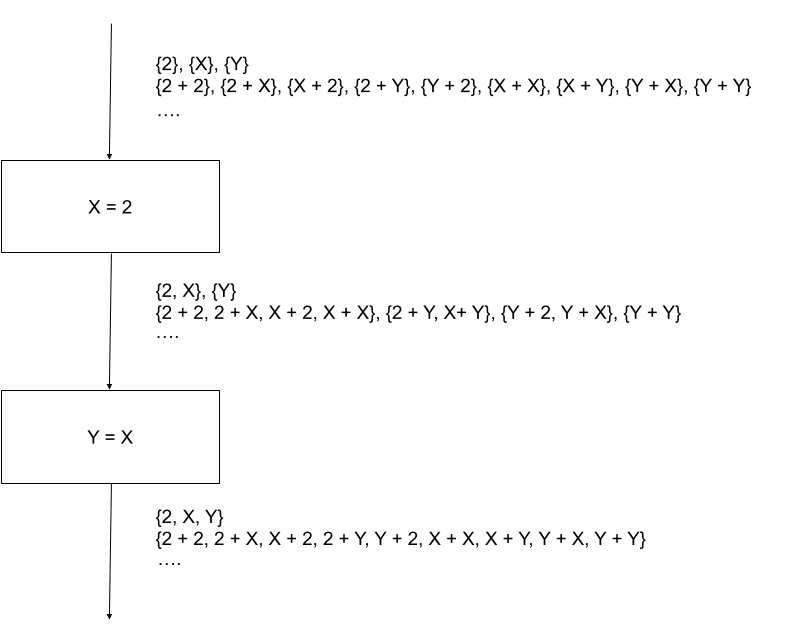
\includegraphics[scale=0.3]{HerbrandEquivalenceTrans.png}
        \caption{Example of Herbrand Equivalence at a \textit{transfer point}}
        \label{fig:HerbrandEquivalenceTrans}
    \end{figure}
\end{frame}

\begin{frame}{Example of Herbrand Equivalence Computation}
    \begin{figure}[!h]
        \centering
        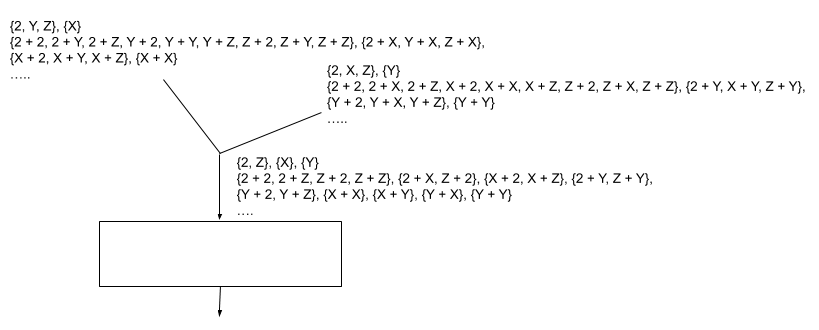
\includegraphics[scale=0.4]{HerbrandEquivalenceConv.png}
        \caption{Example of Herbrand Equivalence at a \textit{confluence point}}
        \label{fig:HerbrandEquivalenceConv}
    \end{figure}
\end{frame}

\begin{frame}{Example of Herbrand Equivalence Computation}
    \begin{figure}[!h]
        \centering
        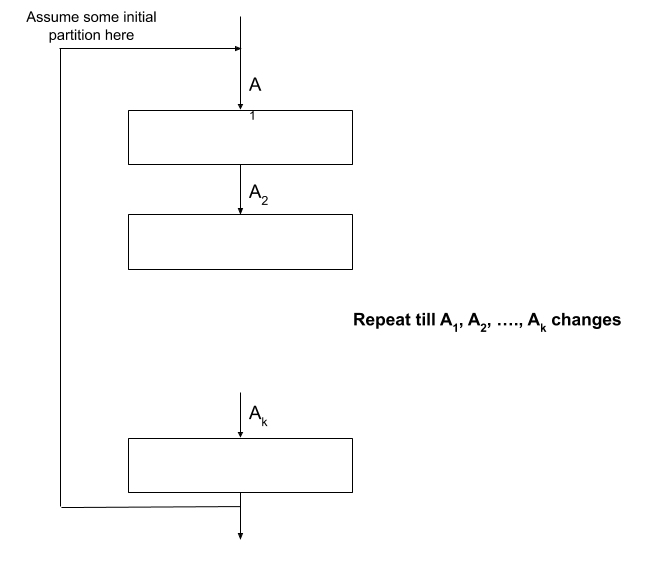
\includegraphics[scale=0.3]{HerbrandEquivalenceLoop.png}
        \caption{Example of Herbrand Equivalence in presence of a loop in the program graph}
        \label{fig:HerbrandEquivalenceLoop}
    \end{figure}
\end{frame}

\begin{frame}{Important points}
    Herbrand equivalence captures only syntactic equivalence, and not semantic
    \begin{itemize}
        \item $2 + 2$ is not equivalent to $4$, they are semantically equivalent and not syntactically 
        \item $X + Y$ is not equivalent to $Y + X$, unless $X$ and $Y$ are equivalent. Because operators are treated as uninterpreted functions, so we cannot consider $+$ to be distributive
    \end{itemize}
\end{frame}

\begin{frame}{Past works}
    \begin{itemize}
        \item There have been several attempts at getting algorithms for computing Herbrand Equivalences
        \item Kildall (in 1973) gave an algorithm to find the Herbrand Equivalence classes. Kildall's algorithm is precise in the sense it finds all the Herbrand Equivalences but is exponential in time and space
        \item Alpern, Wegman and Zadek (in 1998) gave a polynomial time algorithm (AWZ) but it was not able to discover all the Equivalences
        \item Ruthing, Knoop and Steffen (in 1999) improved the AWZ algorithm. It was able to detect more equivalences but was still incomplete
    \end{itemize}
\end{frame}

\begin{frame}{Past works}
    \begin{itemize}
        \item Gulwani and Necula (in 2007) gave an algorithm for finding Herbrand equivalence classes restricted to the program expression. This algorithm was considered complete but later Saleena and Paleri showed that Gulwani's algorithm is not complete for a related problem of global value numbering
        \item The problem is that most of these alogrithms were based on fix point computations. But the classical definition of Herbrand equivalence is not a fix point based definition making it difficult to prove their precision or completeness 
    \end{itemize}
\end{frame}

\begin{frame}{Idea of the Project}
    \begin{itemize}
        \item Babu, Krishnan and Paleri (in 2019) gave a new lattice theoretic formulation of Herbrand equivalences and proved its equivalence to the classical version
        \item Based on their theory they also gave an algorithm to compute \textit{Herbrand equivalences associated with program expressions}
        \item However, the algorithm does not completely follows the theoretical work, so its correctness/precision needs to be established
        \item The task of this project is to implement the algorithm using LLVM framework and benchmark it against the standards
        \item Also, a proof of correctness/precision of the algorithm has to be presented
    \end{itemize}
\end{frame}

\begin{frame}{Work done}
    \begin{itemize}
        \item Read two papers - by Gulwani and Necula\cite{Gulwani}; and by Babu, Krishnan and Paleri\cite{Babu} 
        \item Started experimenting with LLVM, by writing some basic optimization pass
    \end{itemize}
\end{frame}

\begin{frame}{References}
\bibliographystyle{IEEEtran}
\bibliography{citations}
\end{frame}

\end{document}